%
% Documento: Estrutura
%

\chapter{RESULTADOS}
\label{chap:resultados}

Os resultados do sistema IncluiEdu demonstram a viabilidade da integração entre a Inteligência Artificial Generativa e o design inclusivo. As telas reais do sistema, implementadas na Cloudflare, comprovam a aplicação prática dos requisitos levantados na metodologia.

\section{VISÃO GERAL E ORGANIZAÇÃO DO PROFESSOR}

A interface do IncluiEdu foi projetada para oferecer ao docente uma visão clara e organizada de suas responsabilidades. A \autoref{fig:painel_inicial} apresenta o painel inicial do sistema, onde o professor tem acesso rápido às principais funcionalidades.

\begin{figure}[H]
    \centering
    \caption{Tela Inicial do Sistema IncluiEdu}
    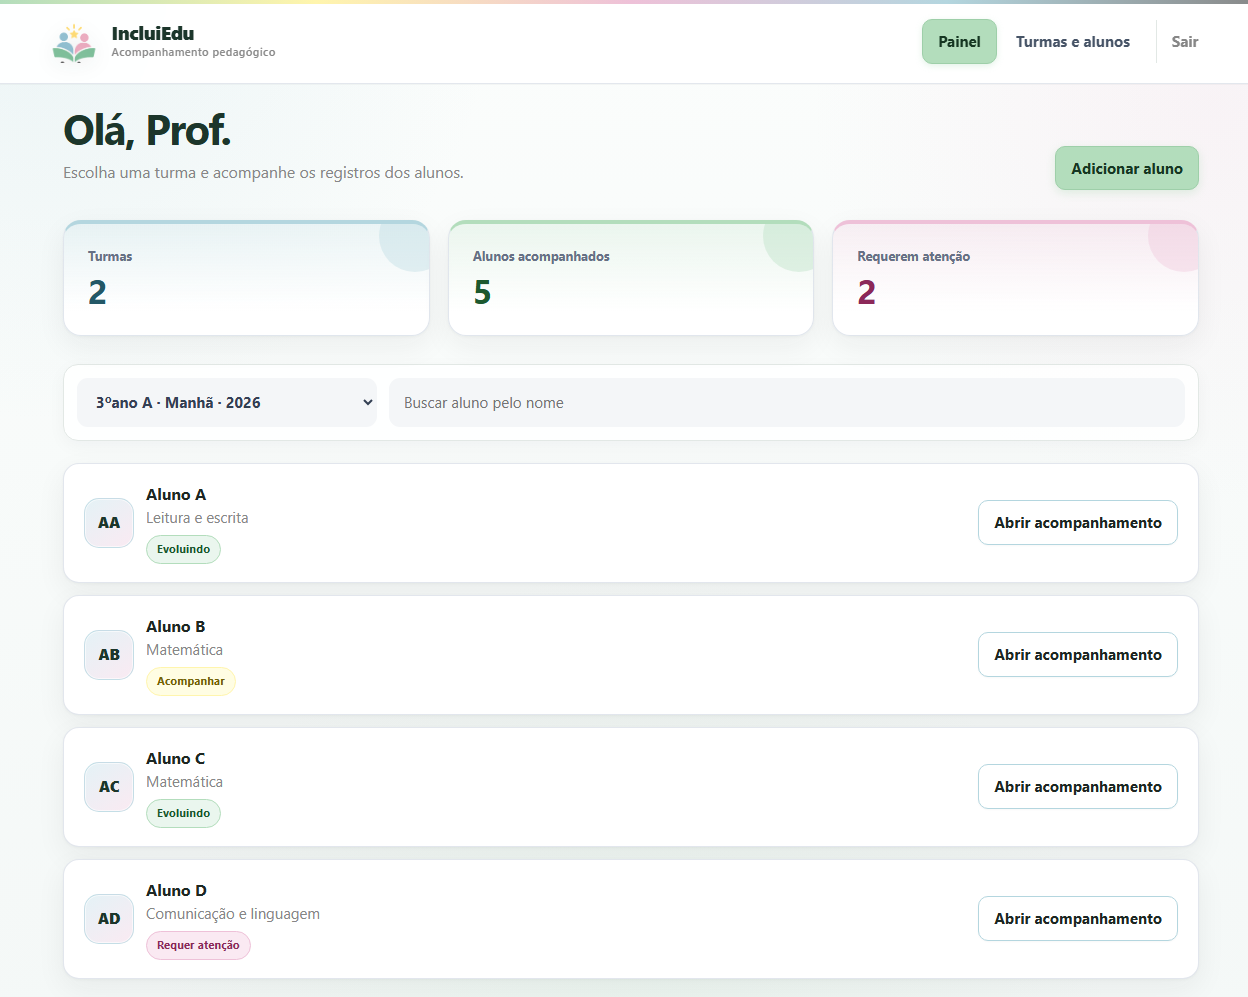
\includegraphics[width=0.9\textwidth]{04-figuras/painel_inicial.png}
    \label{fig:painel_inicial}
    \fonte{Elaborado pelos autores (2026).}
\end{figure}

Observa-se na \autoref{fig:painel_inicial} a aplicação da paleta de cores pastéis, que, conforme discutido na \autoref{sec:interface_carga_cognitiva}, visa reduzir a fadiga visual e a sobrecarga sensorial. A organização limpa da interface atua como um facilitador cognitivo, permitindo que o professor localize rapidamente as ferramentas de que precisa.

Na \autoref{fig:turmas_alunos}, é apresentada a tela de visão geral de turmas. 

\begin{figure}[H]
    \centering
    \caption{Tela de Visão Geral de Turmas}
    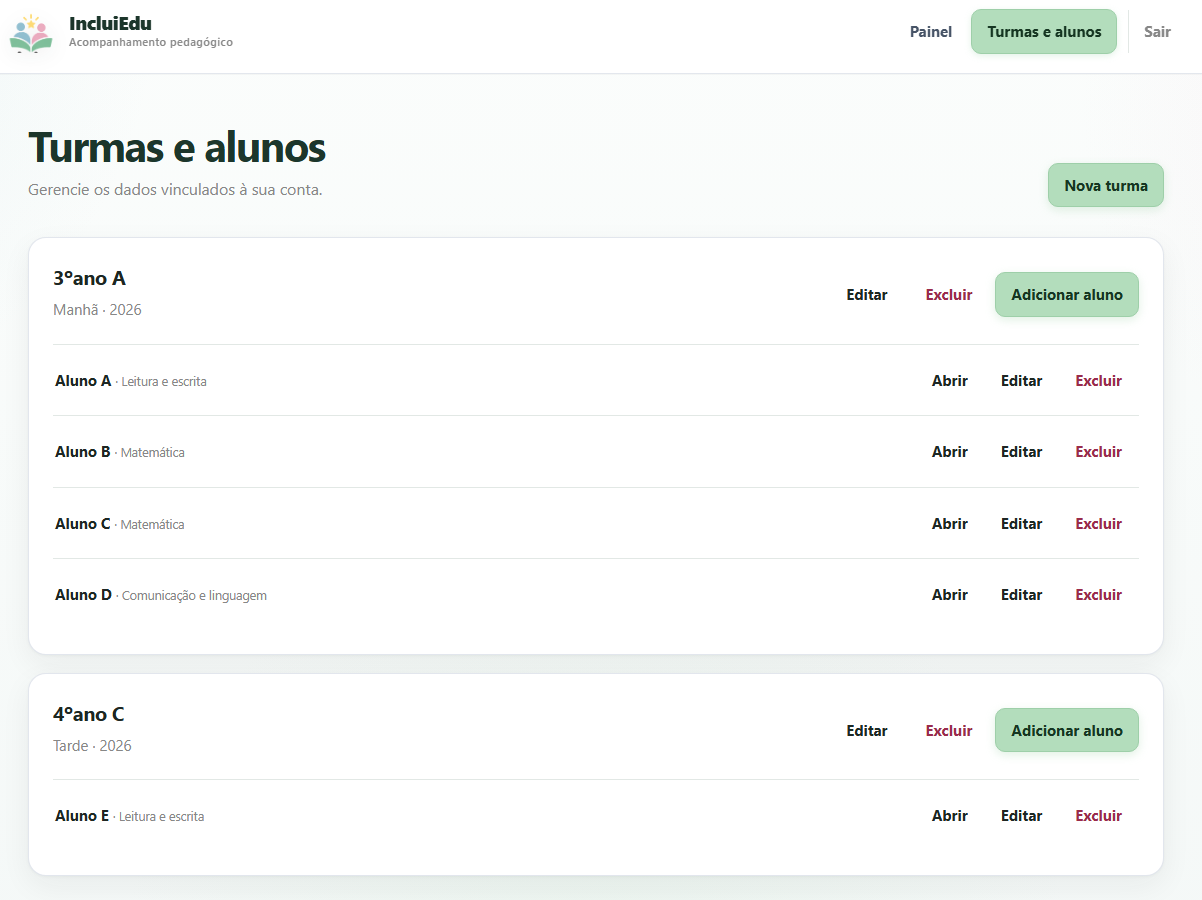
\includegraphics[width=0.9\textwidth]{04-figuras/turmas_alunos.png}
    \label{fig:turmas_alunos}
    \fonte{Elaborado pelos autores (2026).}
\end{figure}

Esta tela (\autoref{fig:turmas_alunos}) permite ao professor gerenciar múltiplos alunos distribuídos em diferentes turmas. A disposição das informações foi pensada para mitigar o problema da sobrecarga docente, apontado por \citeonline{oliveira2025escolas}, ao centralizar o acompanhamento sem a necessidade de navegar por diversas abas ou planilhas externas.

\section{O FLUXO DE GERAÇÃO DE ATIVIDADES PELA INTELIGÊNCIA ARTIFICIAL}

As Figuras \ref{fig:gerar_atividade} e \ref{fig:atv_gerada} apresentam o fluxo central do sistema: a solicitação do professor e a resposta gerada pela IA.

\begin{figure}[H]
    \caption{Fluxo de criação de atividade com Inteligência Artificial}
    \centering
    \begin{subfigure}[b]{0.48\textwidth}
        \centering
        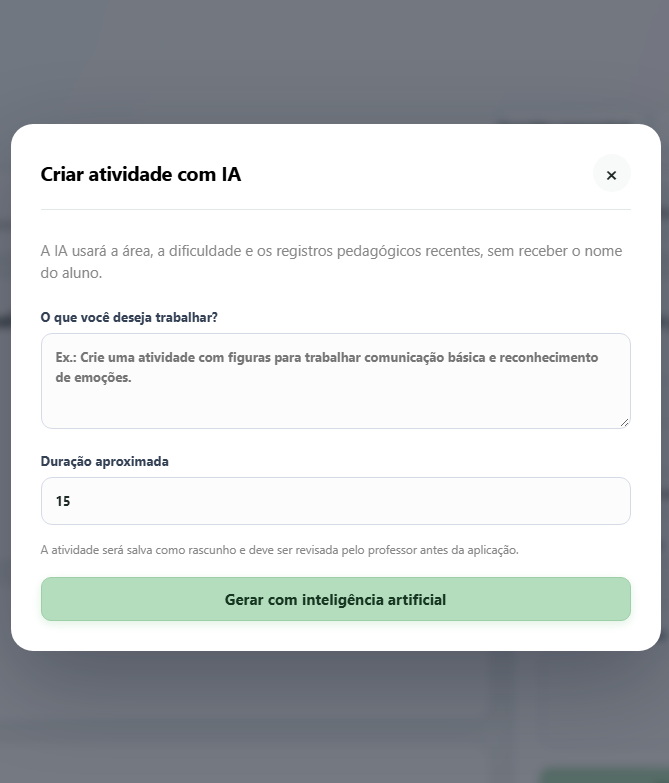
\includegraphics[width=\textwidth]{04-figuras/gerar_atividade.png}
        \caption{Interface de solicitação de atividade}
        \label{fig:gerar_atividade}
    \end{subfigure}
    \hfill
    \begin{subfigure}[b]{0.48\textwidth}
        \centering
        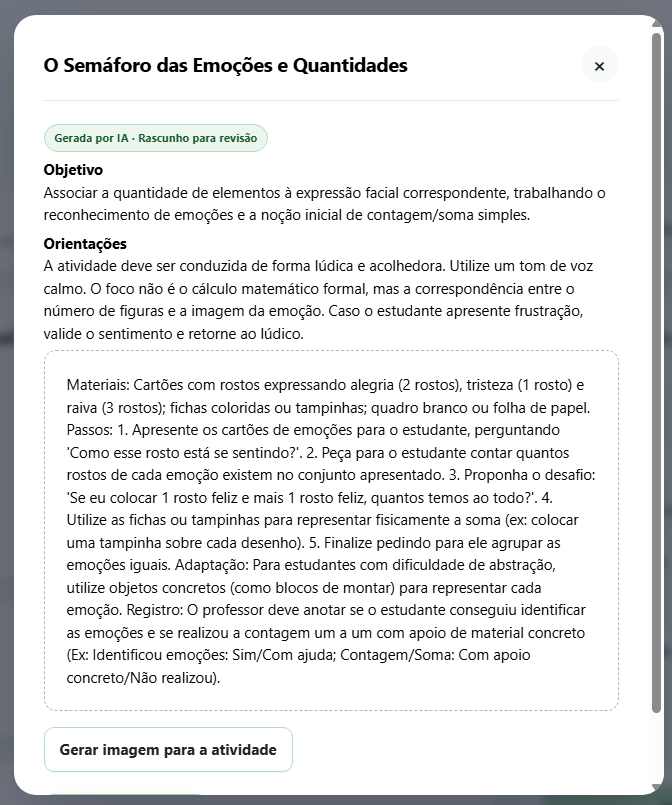
\includegraphics[width=\textwidth]{04-figuras/atv_gerada.png}
        \caption{Atividade gerada com status de rascunho}
        \label{fig:atv_gerada}
    \end{subfigure}
    \label{fig:fluxo-geracao}
    \fonte{Elaborado pelos autores (2026).}
\end{figure}

Observa-se na Figura \ref{fig:gerar_atividade} que o professor informa o tópico desejado (no exemplo, comunicação básica e emoções) e a duração da atividade. Além dessas informações, o sistema utiliza a área de aprendizagem, a dificuldade ou habilidade cadastrada e até cinco registros pedagógicos recentes do estudante, encaminhando esses dados ao modelo de Inteligência Artificial para contextualizar a atividade gerada, conforme descrito na Seção \ref{ia_generativa_apoio}. Os dados encaminhados ao modelo limitam-se ao conteúdo pedagógico dos registros, área de aprendizagem, habilidade observada, nível de autonomia e evidência registrada, sem o nome do estudante, imagem, documento ou qualquer identificador direto, em conformidade com os princípios de finalidade e necessidade previstos na LGPD \cite{brasil2018lgpd} e com os requisitos RNF07 e RNF08. A Figura \ref{fig:atv_gerada} apresenta o retorno da IA, que gerou uma atividade lúdica intitulada "O Semáforo das Emoções e Quantidades". Nota-se a aplicação prática da barreira de segurança pedagógica discutida na Subseção \ref{ia_generativa_apoio}: o sistema destaca a identificação "Gerada por IA - Rascunho para revisão", permitindo que o professor avalie o conteúdo antes de aplicá-lo ao aluno.

\section{ORGANIZAÇÃO VISUAL E SINALIZAÇÃO CROMÁTICA}

A Figura \ref{fig:acompanhamento_aluno} ilustra a tela de acompanhamento individual do aluno, onde são aplicados os conceitos de design inclusivo.

\begin{figure}[H]
    \centering
    \caption{Tela de Acompanhamento do Aluno}
    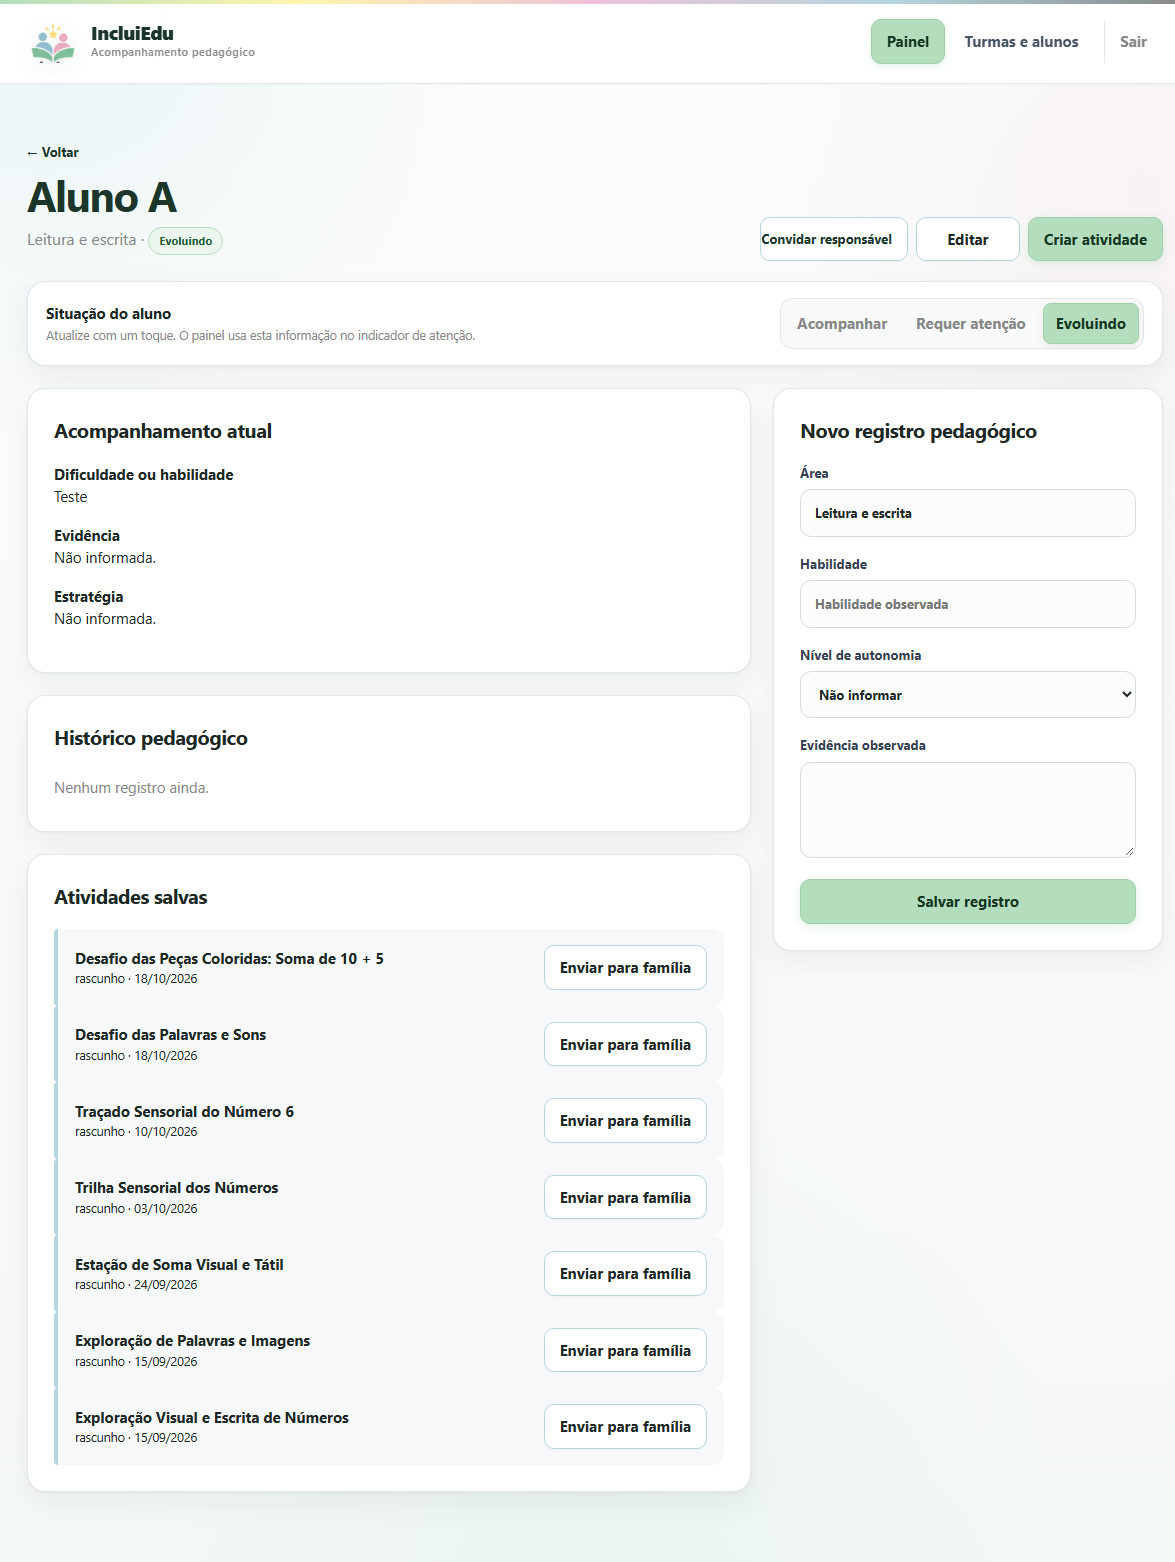
\includegraphics[width=0.8\textwidth]{04-figuras/acompanhamento_aluno.png}
    \label{fig:acompanhamento_aluno}
    \fonte{Elaborado pelos autores (2026).}
\end{figure}

Conforme observado na Figura \ref{fig:acompanhamento_aluno}, a interface utiliza uma paleta de cores pastéis e \textit{badges} de sinalização cromática para indicar a situação do estudante. Como fundamentado na \autoref{sec:interface_carga_cognitiva}, essa escolha visual não é meramente estética, mas atua como um filtro cognitivo, permitindo que o professor identifique alunos que necessitam de maior atenção sem sobrecarregar seu processamento visual.


\chapter{CONCLUSÃO}

Este trabalho respondeu à pergunta de pesquisa, como apoiar o professor do ensino fundamental na criação de atividades adaptadas para alunos neurodivergentes sem retirar seu controle pedagógico e ético, por meio do desenvolvimento do IncluiEdu, sistema web que usa IA Generativa como apoio à decisão docente, e não como substituto do professor.

Quanto aos objetivos, todos foram alcançados, com exceção da validação com professores. A identificação dos desafios docentes foi feita no \autoref{chap:fundamentacao}, com base na literatura sobre formação insuficiente e precariedade de recursos. Os requisitos, a arquitetura e o modelo de banco de dados foram definidos e materializados nos diagramas da \autoref{sec:modelagem-sistema}. A interface neuroinclusiva foi implementada e comprovada nos resultados, com paleta pastel e sinalização cromática, conforme a \autoref{sec:interface_carga_cognitiva}. A integração com a IA Generativa via Cloudflare Workers AI é demonstrada na \autoref{fig:fluxo-geracao}. O mecanismo de segurança pedagógica, atividades sempre salvas como rascunho, exigindo revisão do professor, foi implementado e constitui o diferencial ético do sistema. Por fim, a validação por testes manuais confirmou o funcionamento dos fluxos de cadastro, acompanhamento e geração na \autoref{sec:testes-validacao}, mas não envolveu professores reais, o que se configura como limitação.

Conclui-se que o IncluiEdu responde à pergunta de pesquisa de forma viável: reduz parte da sobrecarga de planejamento ao gerar rascunhos de atividades adaptadas, preservando a autonomia e a responsabilidade ética do educador. Trata-se, contudo, de uma contribuição inicial, cujas limitações e desdobramentos seguem abaixo.

\section{LIMITAÇÕES}

A principal limitação é a ausência de avaliação com professores em contexto real: a validação foi apenas técnica e manual, sem aplicação com docentes nem avaliação de usabilidade com o público-alvo. Além disso, a qualidade pedagógica das atividades geradas não foi medida de forma sistemática, sendo tratada apenas pela revisão humana. Há também os riscos de alucinação da IA Generativa, mitigados pela validação docente, mas sem filtros automáticos de consistência. Por fim, o sistema armazena dados sensíveis de alunos: embora a persistência seja realizada no banco de dados Cloudflare D1, cuja segurança é de responsabilidade da infraestrutura do provedor, não foi realizada auditoria formal de conformidade com a LGPD nem verificação independente das políticas de segurança e privacidade da Cloudflare. A validação também se restringiu a testes manuais, sem testes automatizados ou de segurança.

\section{TRABALHOS FUTUROS}

Como desdobramentos, propõe-se: avaliar o sistema com professores reais, mensurando a redução da sobrecarga, desenvolver instrumentos, com especialistas, para medir a qualidade pedagógica das atividades, aprimorar o mecanismo de filtros para a mitigação de alucinações da IA, políticas de tratamento dos dados dos alunos, incorporar testes automatizados e de segurança, ampliar mecanismos internos do sistema para melhor atender os professores e pais.